\documentclass[xcolor=x11names,compress,aspectratio=169]{ctexbeamer}
\usetheme{Darmstadt} 
\useoutertheme[subsection=false,footline=authortitle]{miniframes}
\setbeamertemplate{navigation symbols}{} 
\logo{
\includegraphics[height=0.07\textwidth]{Figure/sjtu-red.png}}
\setbeamertemplate{background}{
\includegraphics[width=\paperwidth]{Figure/sjtu-miao.png}}
\usepackage{datetime}
\newdateformat{mydate}{\monthname[\THEMONTH] \THEDAY, \THEYEAR}
%\usefonttheme[onlymath]{serif}


\usepackage{fontspec}
\usefonttheme{serif}
\setbeamercolor*{lower separation line head}{bg=DeepSkyBlue4} 
\setbeamercolor*{normal text}{fg=black,bg=white} 
\setbeamercolor*{alerted text}{fg=red} 
\setbeamercolor*{example text}{fg=black} 
\setbeamercolor*{structure}{fg=DeepSkyBlue4,bg=white} 

\setbeamercolor*{palette tertiary}{fg=black,bg=black!10} 
\setbeamercolor*{palette quaternary}{fg=black,bg=black!10} 

%footline
\setbeamercolor{author in head/foot}{fg=white,bg=}
\setbeamercolor{title in head/foot}{fg=white,bg=}
\setbeamercolor{date in head/foot}{fg=black,bg=}


\makeatletter
\setbeamertemplate{footline}
{%
    \setbox\beamer@tempbox=\hbox{%
        \begin{beamercolorbox}[wd=.333333\paperwidth,ht=2.25ex,dp=1ex,center]{author in head/foot}%
            \usebeamerfont{author in head/foot}  \rmfamily Racheus Zhao(SJTU)
        \end{beamercolorbox}%
        \begin{beamercolorbox}[wd=.333333\paperwidth,ht=2.25ex,dp=1ex,center]{title in head/foot}%
            \usebeamerfont{title in head/foot} \rmfamily ME4918-Graduation Project
        \end{beamercolorbox}%
        \begin{beamercolorbox}[wd=.333333\paperwidth,ht=2.25ex,dp=1ex,right]{date in head/foot}%
            \usebeamerfont{date in head/foot} \rmfamily \insertshortdate{}\hspace*{2em}
            \insertframenumber{} / \inserttotalframenumber\hspace*{2ex} 
        \end{beamercolorbox}%
    }%
    \vskip0pt%
        \begin{pgfpicture}{0pt}{0pt}{\paperwidth}{0cm}%
            \usebeamercolor{frametitle right}%
            \pgfpathrectangle{\pgfpointorigin}{\pgfpoint{\paperwidth}{3.5ex}}%
            \pgfusepath{clip}%
            \pgftext[left,base]{\pgfuseshading{beamer@frametitleshade}}%
        \end{pgfpicture}%
    \beamer@tempdim=\ht\beamer@tempbox%
    \advance\beamer@tempdim by 0.95ex%
    \vskip-\beamer@tempdim%
    \box\beamer@tempbox%
    }  
\makeatother


\colorlet{titleright}{yellow!10!white}
\colorlet{titleleft}{DeepSkyBlue4}
\colorlet{titlemid}{green!60!blue}

\makeatletter

\pgfdeclarehorizontalshading[titleleft,titleright]{beamer@frametitleshade}{\paperheight}{%
        color(0pt)=(titleleft);
        color(.5\paperwidth)=(titlemid);
        color(\paperwidth)=(titleright)
}

\AtBeginDocument{
    \pgfdeclareverticalshading{beamer@topshade}{\paperwidth}{%
        color(0pt)=(bg);
        color(4pt)=(black!50!bg)    
    }
}


\renewcommand{\(}{\begin{columns}}
\renewcommand{\)}{\end{columns}}
\newcommand{\<}[1]{\begin{column}{#1}}
\renewcommand{\>}{\end{column}}


\usepackage{listings}

\lstset{
    language=C++, % 设置语言为C++
    basicstyle=\ttfamily\small, % 设置代码字体样式
    numbers=left, % 在左侧显示行号
    numberstyle=\tiny\color{gray}, % 行号样式
    keywordstyle=\color{blue}, % 关键字颜色
    commentstyle=\color{green!60!black}, % 注释颜色
    stringstyle=\color{red}, % 字符串颜色
    breaklines=true, % 自动换行
    columns=flexible,%不随便添加空格,只在已经有空格的地方添加空格,
%如果想要添加空格使用fixed作为参数(这是默认的),如果坚决不添加空格使用fullflexible作为参数
    frame=single, % 显示边框
    backgroundcolor=\color{lightgray!10}, % 背景色
}



\title{ Graduation Project  (ME4918)\\
  \textbf{Weekly Report(X)}}

\author{\selectfont\kaishu 赵四维}
 
\institute
{
   Institute of Robotics,\\
   School of Mechanical Engineering,SJTU 
}

\date{\mydate\today}


\begin{document}

\maketitle

\AtBeginSection[]
{
  \begin{frame}
    \frametitle{Table of Contents}
    \tableofcontents[currentsection,hideallsubsections]
  \end{frame}
}

\section{Figure and Notes}
\subsection{Figure and Notes}

\begin{frame}{Figure and Notes}
In Simulink, you can import models from other modeling environments, such as Solidworks.
\begin{figure}

\includegraphics[width=0.8\textwidth]{Figure/logo.png}
\end{figure}

Save the modeling file in XML format or URDF format, set a reasonable rotation coordinate system, and import it into Simulink for simulation.
\end{frame}

\section{Chinese Characters}
\subsection{中文测试}
\begin{frame}{中文测试}
\vspace{-2cm}
\hspace{3cm}
\begin{itemize}
  \item 邓紫棋
  \item 林俊杰
\end{itemize}

\begin{center}
  \textbf{手心的蔷薇(加粗)}

  \selectfont \kaishu 刺伤而不自觉(楷书)
  
  \selectfont \heiti 你值得被疼爱(黑体)
  
  \selectfont \fangsong 你懂我的期待(仿宋)
\end{center}

\begin{block}{代表作展示}
  \begin{itemize}
    \item 邓紫棋:《倒数》,《多远都要在一起》
    \item 林俊杰:《修炼爱情》,《可惜没如果》
  \end{itemize}
\end{block}

\end{frame}  

\section{Mathematical Formula}
\subsection{Mathematical Formula}
\begin{frame}{Mathematical Formula}
\begin{block}{Mathematical Formula}
  \begin{equation}
    \begin{aligned}
      \dot{x} &= Ax + Bu \\
      y &= Cx + Du
    \end{aligned}
  \end{equation}
\end{block}

对于机械臂的拉格朗日动力学方程,可以写成如下形式:
\begin{equation}
  \begin{aligned}
    \frac{d}{dt}(\frac{\partial L}{\partial \dot{q}_i}) - \frac{\partial L}{\partial q_i} &= Q_i
  \end{aligned}
\end{equation}

Where Lagrangian $L$ is defined as:
\begin{equation}
  \begin{aligned}
    L &= T - V
  \end{aligned}
\end{equation}
\end{frame}

\section{Coding Environment}
\subsection{Coding Environment}
\begin{frame}{Coding Environment}
import numpy as np

\begin{figure}
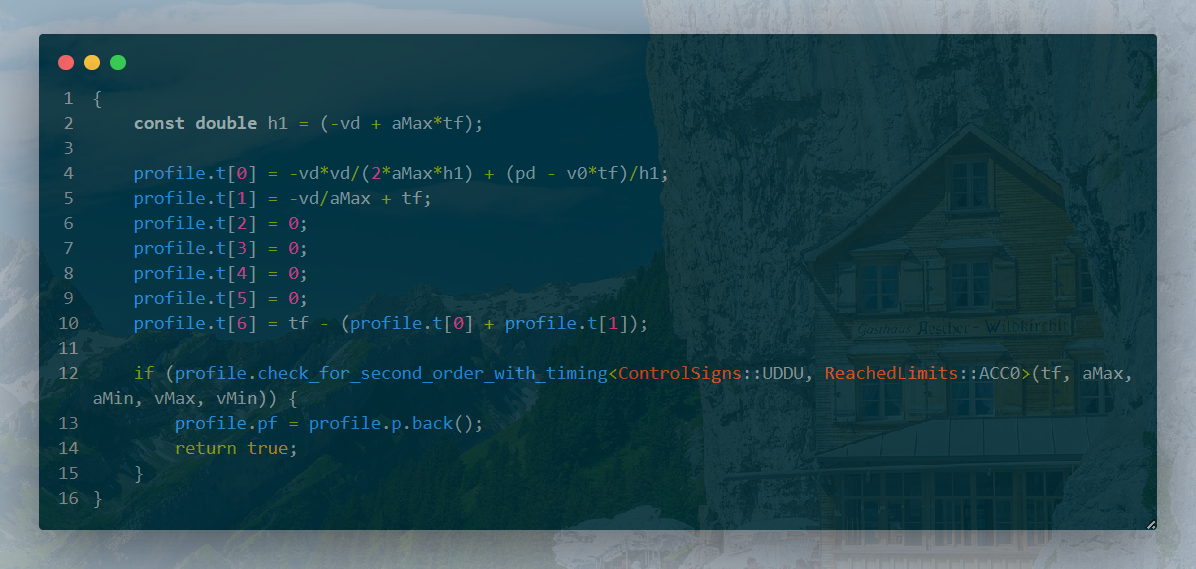
\includegraphics[width=0.8\textwidth]{Figure/code.png}
\end{figure}

CodeSnap + Figure 清晰度不太高


\end{frame}


\begin{frame}[fragile] % 使用fragile选项以在frame内使用lstlisting环境
  \frametitle{lstlisting Environment}
  
  Here is a sample C++ code snippet:\\
  
  \begin{lstlisting}[caption={Sample C++ Code}]
  #include <iostream>
  
  int main() {
      std::cout << "Hello, Beamer!" << std::endl;
      return 0; //test
  }
  \end{lstlisting}
  
  \end{frame}

  
  \begin{frame}
    \begin{center}
      \vspace{1cm}
      \Huge \textbf{Thanks for listening!}
      \vspace{2cm}
      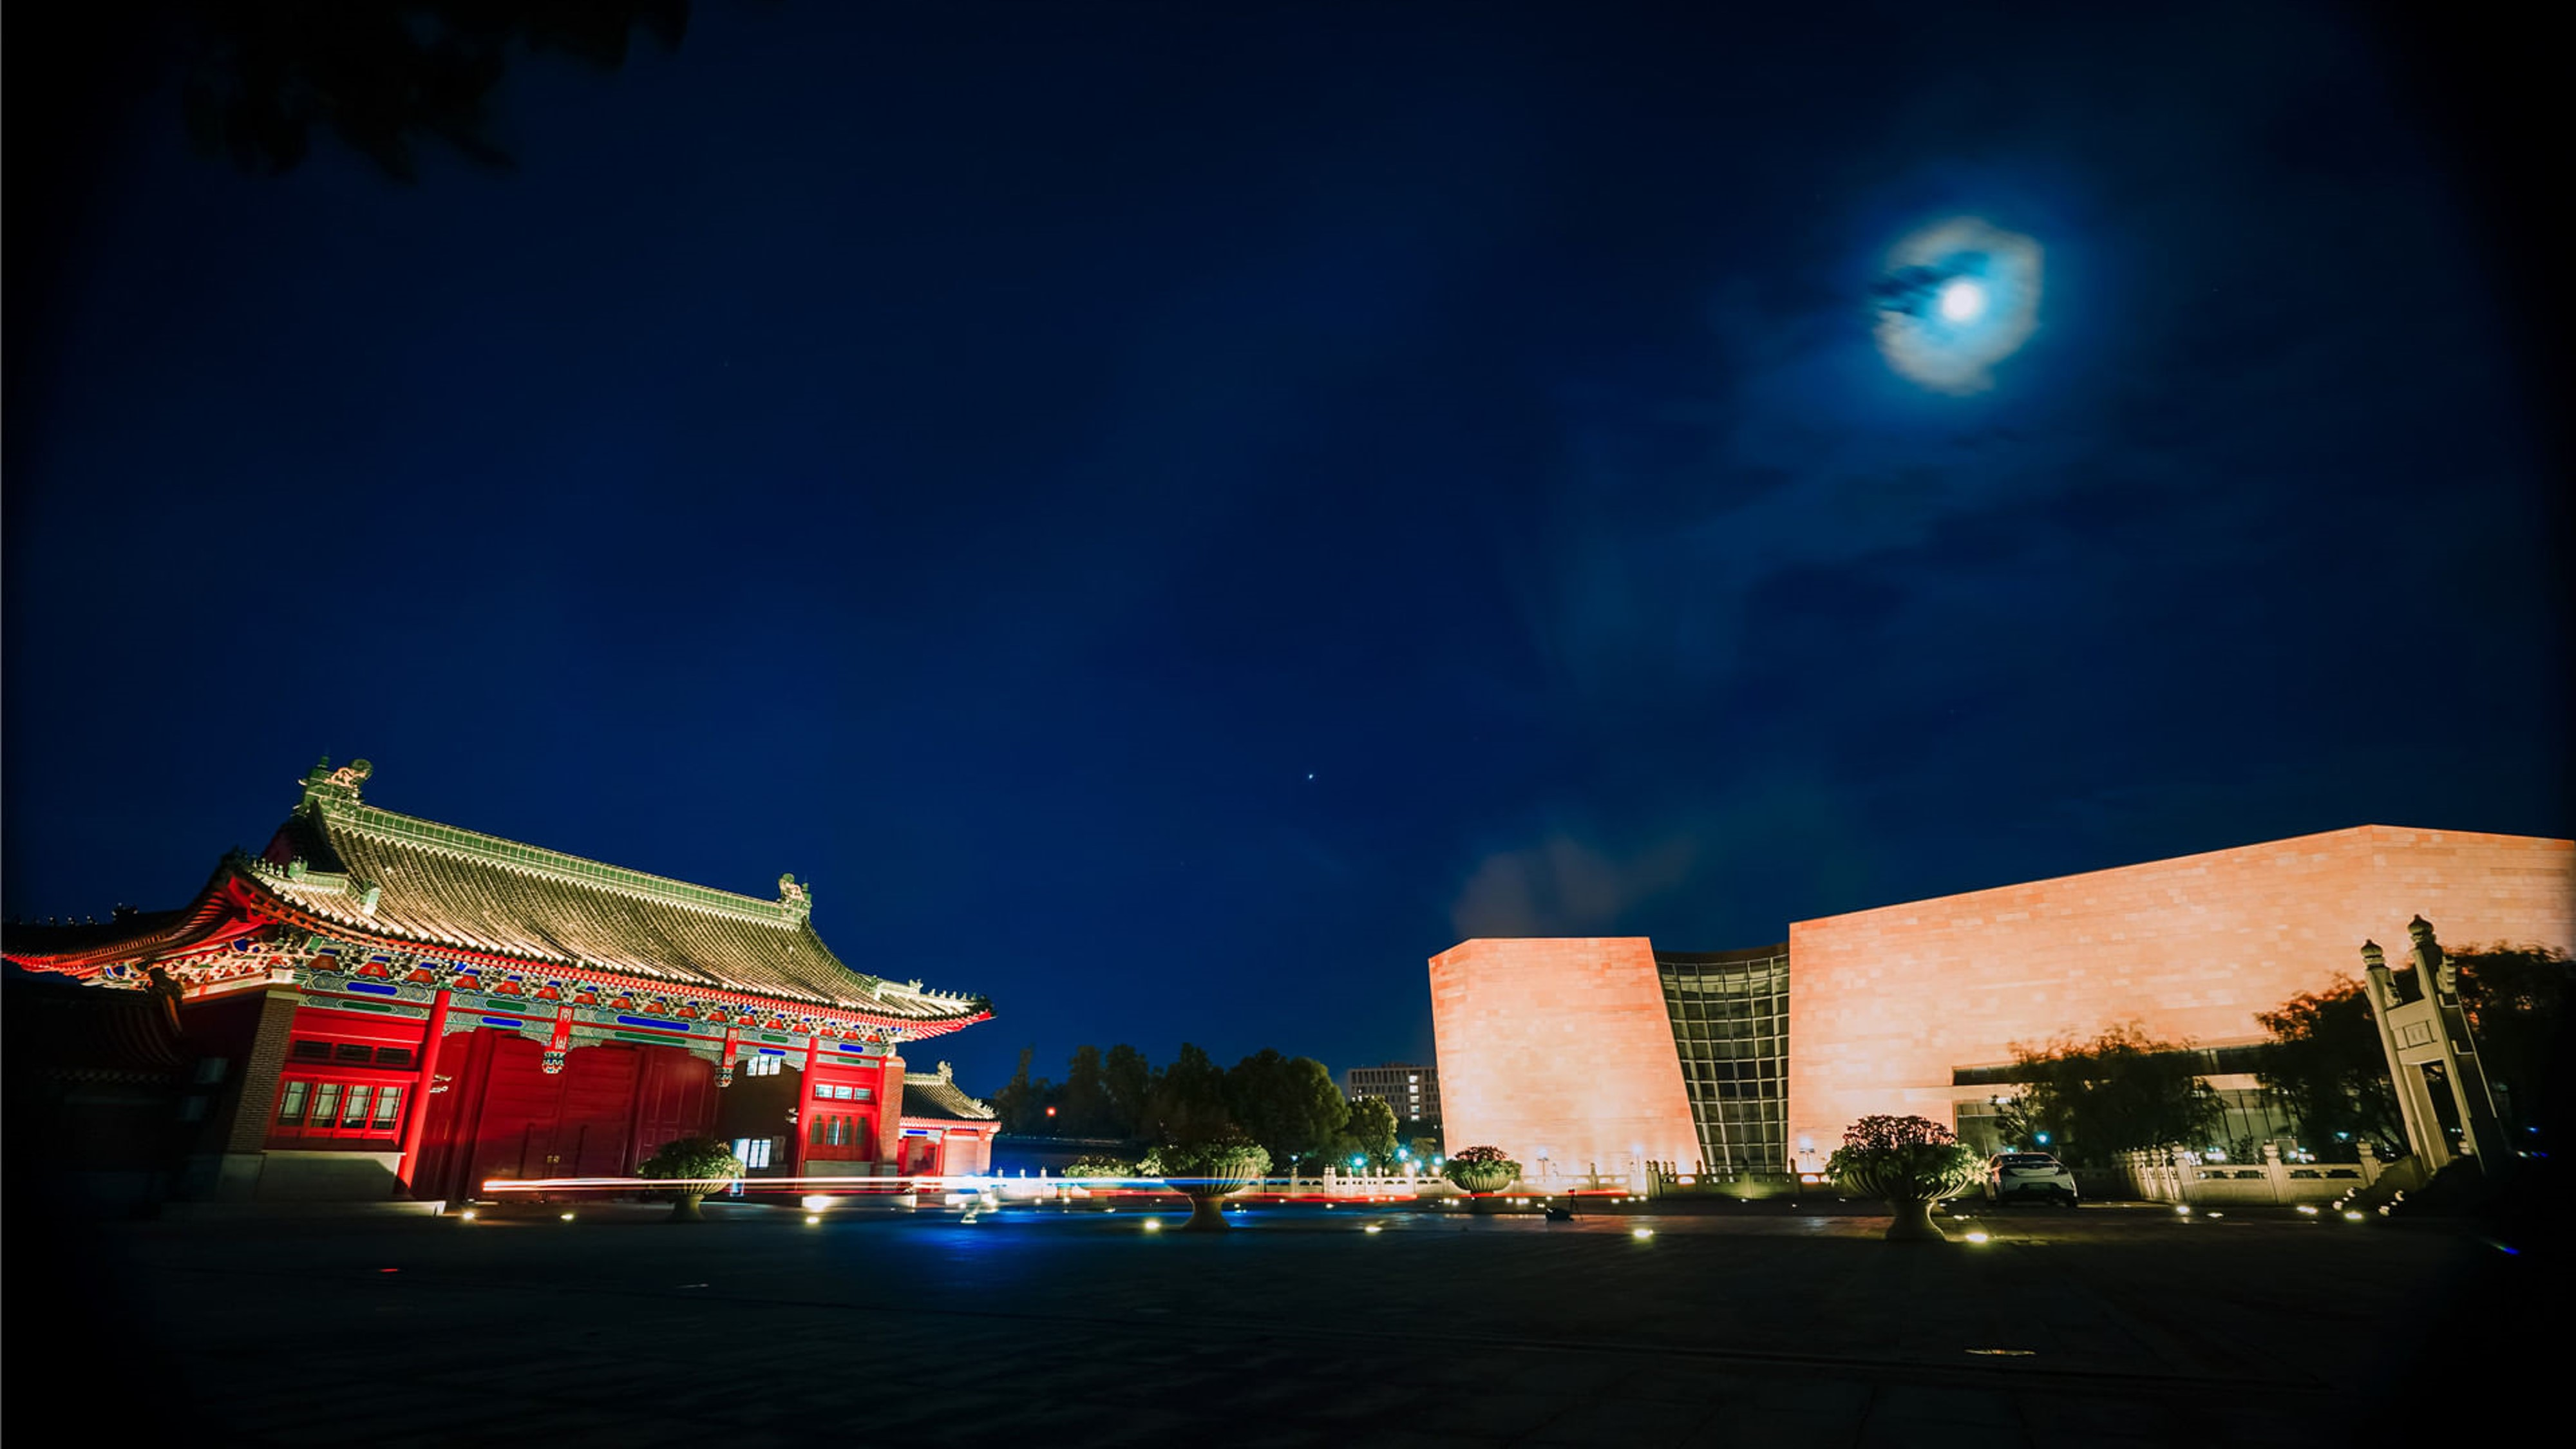
\includegraphics[width=0.8\textwidth]{Figure/siyuan.jpg} % Optional: Add an image
    \end{center}
  \end{frame}
\end{document}